%%%%%%%%%%%%%%%%%%%%%%%%%%%%%%%%%%%%%%%%%%%%%%%%%%%%%%%%%%%%%%%%%%%%%%%%%%%%%%%
% Chapter 2: Desarrollo
%%%%%%%%%%%%%%%%%%%%%%%%%%%%%%%%%%%%%%%%%%%%%%%%%%%%%%%%%%%%%%%%%%%%%%%%%%%%%%%

%++++++++++++++++++++++++++++++++++++++++++++++++++++++++++++++++++++++++++++++

En el capítulo anterior se ha descrito el estado del arte actual y se ha definido el Trabajo de Fin de Máster, especificado los objetivos, actividades a desarrollar y las tecnologías empleadas para su desarrollo. A continuación, se describirá la metodología de trabajo seguida.

%++++++++++++++++++++++++++++++++++++++++++++++++++++++++++++++++++++++++++++++

\section{Metodología usada}
\label{2:sec:1}

Se ha llevado a cabo una metodología de trabajo ágil, común en el campo de la Ingeniería Informática, con reuniones quincenales en las que se definían una serie de tareas u objetivos (iteración) y que se presentaban la siguiente quincena. 
De este modo, con la entrega de prototipos funcionales de la aplicación, se han ido testeando, corrigiendo y mejorando las 
funcionalidades, al mismo tiempo que detectando problemas no contemplados en las fases previas de diseño.

Esta metodología, además, ha propiciado la generación de ideas que se han traducido en nuevas características.


%---------------------------------------------------------------------------------
\subsection{GitHub}
\label{subsec:2.1.1}

Para llevar a cabo esta metodología, se ha usado GitHub como herramienta de Control de Versiones (CVS).
Todo el código implementado se alojaba en dicha herramienta, permitiendo así su cómoda modificación y actualización.

\begin{figure}[H]
\begin{center}
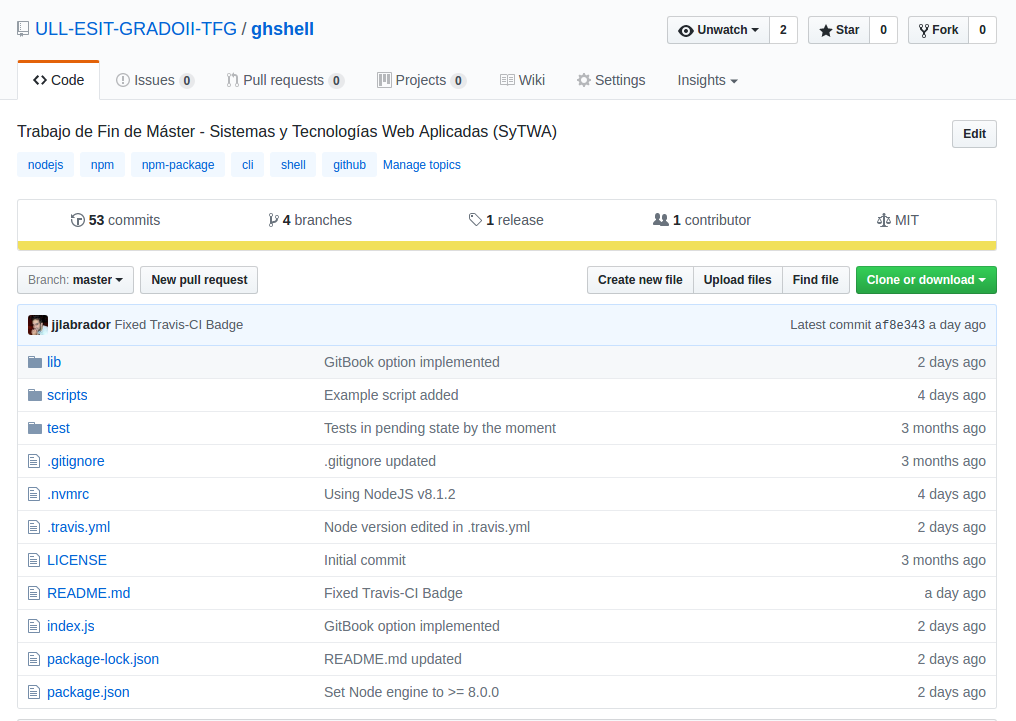
\includegraphics[width=0.9\textwidth]{images/github1}
\caption{Captura del repositorio del paquete NPM en GitHub}
\label{fig:github1}
\end{center}
\end{figure}

El trabajo se dividía en ramas, de modo que la versión estable de la aplicación (rama master) quedara aislada de la 
versión en desarrollo (rama develop) y de la rama experimental (rama test).


\begin{figure}[H]
\begin{center}
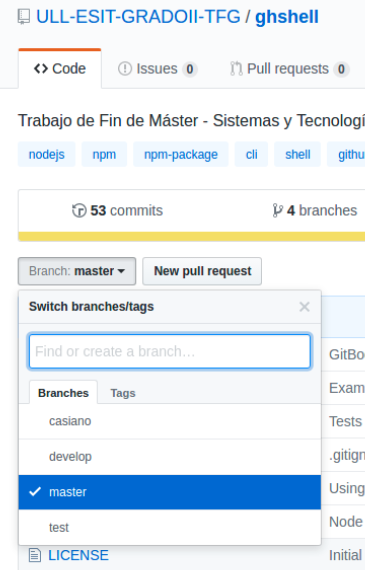
\includegraphics[width=0.47\textwidth]{images/github2}
\caption{Ramas del repositorio}
\label{fig:github2}
\end{center}
\end{figure}


La documentación adicional para llevar a cabo los desarrollos de cada iteración, así como los problemas detectados, se anotaban en el apartado de issues con el fin de que quedara constancia de ello y se reflejara el estado en el que se encontraba cada uno.

\begin{figure}[H]
\begin{center}
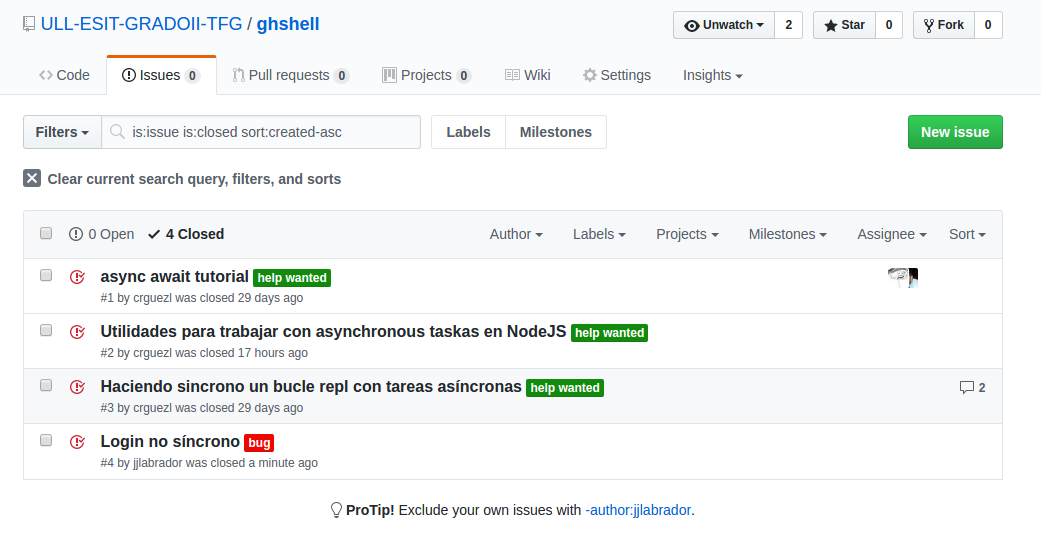
\includegraphics[width=1\textwidth]{images/github3}
\caption{Apartado de issues}
\label{fig:github3}
\end{center}
\end{figure}

%---------------------------------------------------------------------------------
\subsection{Travis-CI}
\label{subsec:2.1.2}

Como herramienta de integración continua, se ha utilizado Travis-CI, con el fin de asegurarnos el despliegue de la aplicación era satisfactorio tras cada cambio subido a la herramienta de control de versiones (GitHub).

\begin{figure}[H]
\begin{center}
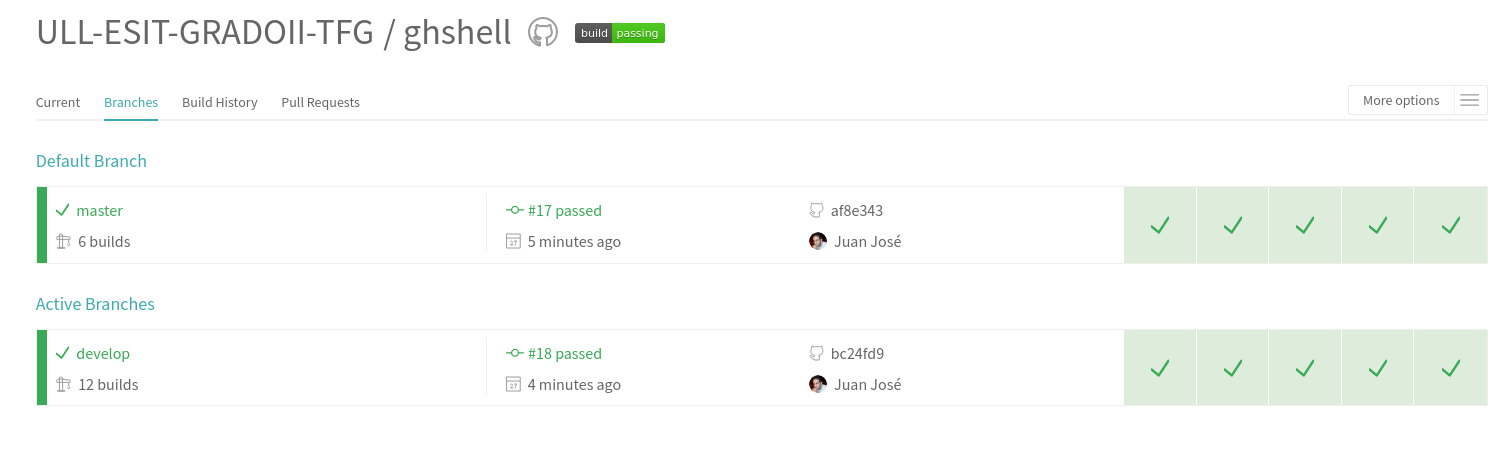
\includegraphics[width=1.1\textwidth]{images/travis-ci}
\caption{Herramienta de integración continua}
\label{fig:travisci}
\end{center}
\end{figure}

%---------------------------------------------------------------------------------
\subsection{Experiencia de usuario}
\label{subsec:2.1.3}

Por otra parte, el tutor del Trabajo de Fin de Máster ha hecho pruebas reales con el resultado de cada iteración. De este modo, se comprobaba el funcionamiento de la aplicación en un entorno real y se recibía un valioso feedback para corregir problemas o hacer mejoras en las siguientes iteraciones.
